\pagestyle{fancy}
\chapter{Quantization Techniques}
\label{chap:Vector quantization in VBDMS}
This chapter explores \textbf{vector quantization} techniques, which arise from the need to optimize the memory and disk footprint of \textbf{VDBMS}. By reducing storage requirements, these techniques enable more efficient resource usage and higher \textbf{queries per second (QPS)}. However, this efficiency comes at the expense of search accuracy, introducing a trade-off between precision and performance. Quantization methods can be broadly categorized into two types: those that reduce dimensionality, such as \textbf{Product Quantization}, and those that approximate values, such as \textbf{Scalar Quantization} and \textbf{Binary Quantization}.

\section{Product Quantization}
\textbf{Product Quantization (PQ)} reduces memory usage by restricting vector representation, making storage and retrieval more efficient. The process begins by dividing the original vector into several smaller sub-vectors of equal size, and the greater the number of sub-vectors, the lower the compression rate, as more data points need to be stored. Each sub-vector represents a separate subspace, where we apply a clustering algorithm associated with its closest centroid.
\begin{figure}[h]
    \centering
    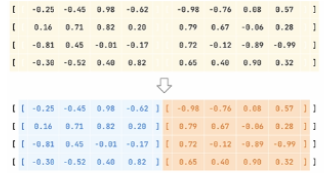
\includegraphics[width=0.65\textwidth]{IMAGES/immagine_2025-02-27_122846884.png}
    \caption[Product Quantization.]{Product Quantization. Source: DeepLearning.AI.\footnotemark[1]}
    \label{fig:PQ}
\end{figure}
\footnotetext[1]{\url{https://learn.deeplearning.ai/courses/retrieval-optimization-from-tokenization-to-vector-quantization/lesson/1/introduction}}

\begin{description}
\item[\textbf{Codebook}:] It refers to the collection of all centroids of a specific subspace.
\end{description}

Formally, the \textbf{product quantization} process goes as follows:
\begin{enumerate}
    \item Decomposing the vector \( \mathbf{x} \) into subvectors \( k \): \( \mathbf{x} = [\mathbf{x}_1, \mathbf{x}_2, \dots, \mathbf{x}_k] \), where each subvector \( \mathbf{x}_i \in \mathbb{R}^{d_i} \) and \( \sum_{i=1}^k d_i = d \).
    \item Quantizing each sub-vector \( \mathbf{x}_i \) independently using a \textbf{codebook} \( C_i = \{c_{i1}, c_{i2}, \dots, c_{iM}\} \), where \( M \) is the number of centroids for each sub-vector.
    \item The quantized vector is then the concatenation of the indices of the chosen codewords: \( \mathbf{q} = [q_1, q_2, \dots, q_k] \), where \( q_i \) is the index of the nearest codeword in \( C_i \).
\end{enumerate}


\subsection{Centroid Generation}
As for generating centroids, VDBMSs like Weaviate and Qdrant rely on the widely used encoder algorithm \textbf{K-means}. It defines a \textbf{K} parameter, which is the number of partitions (also referred to as tiles) we want for our subvector space. The algorithm starts by assigning \textbf{K} random centroids within the dataset, then iteratively assigns the closest vectors to them, recalculating the cluster using the mean of the residing vectors. The algorithm stops when the centroids have stabilized or a maximum number of iterations have been reached.
\begin{figure}[h]
    \centering
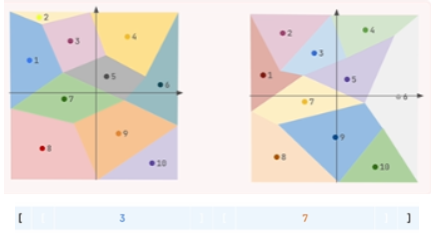
\includegraphics[width=0.7\textwidth]{IMAGES/immagine_2025-02-27_123033735.png}
    \caption[Partitioned Vector Space.]{Partitioned Vector Space. Source: DeepLearning.AI.\footnotemark[1]}
    \label{fig:PQ}
\end{figure}
Another algorithm used to partition the subvector space is the \textbf{Tile encoder}. This algorithm aims to resolve one of the main limitations of K-means, which is the tendency for centroids to become outdated over time as new vectors join the collection. This results in some centroids becoming more populated than others. 

The Tile encoder addresses this issue by employing the Cumulative Density Function (CDF), denoted as \textbf{CDF}(x). Given our data collection, it returns the probability (a value from 0 to 1) that a data point is less than or equal to \(x\). Using the formula \(\text{code}(x) = \text{CDF}(x) \times c\) (where c is the number of codes/clusters we need), we determine the cluster to which the data point \(x\) belongs. 


\section{Scalar Quantization}
\textbf{Scalar Quantization} reduces the precision of numerical values by mapping continuous floating-point numbers to a fixed set of discrete levels. Typically, this involves converting each dimension from a 32-bit floating-point representation to an 8-bit integer. The process begins by analyzing the data to determine the range, setting boundaries based on the minimum and maximum values from a training set. The range is then divided into a fixed number of intervals (e.g., 256 for 8-bit quantization), with each value assigned to the nearest bucket. The resulting integer represents the corresponding bucket, enabling a more compact and efficient representation while preserving as much information as possible within the given bit constraint.
\begin{figure}[h]
    \centering
    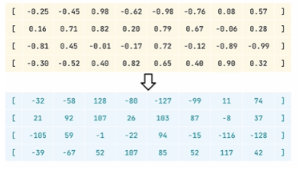
\includegraphics[width=0.65\textwidth]{IMAGES/immagine_2025-02-27_123316646.png}
    \caption[Scalar Quantization.]{Scalar Quantization. Source: DeepLearning.AI.\footnotemark[1]}
    \label{fig:SQ}
\end{figure}

\section{Binary Quantization}
\textbf{Binary Quantization} consists of converting a floating point to a binary representation, taking the quantization to the extreme by transitioning from a 32-bit representation to a single bit. By sacrificing a huge amount of information and distance calculation accuracy, \textbf{Binary Quantization} excels by having a minor memory and disk footprint. This technique is very susceptible to \textbf{oversampling}(vectors with the same compressed representation), while being the fastest.
\begin{figure}[h]
    \centering
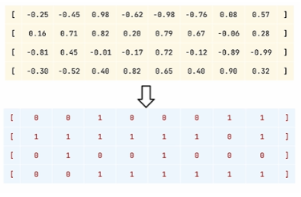
\includegraphics[width=0.65\textwidth]{IMAGES/immagine_2025-02-27_123438887.png}
    \caption[Binary Quantization.]{Binary Quantization. Source: DeepLearning.AI.\footnotemark[1]}
    \label{fig:BQ}
\end{figure}

\section{Overfetching and Rescoring}
To mitigate the limitations of vector quantization, vector database management systems (\textbf{VDBMSs}) employ \textbf{overfetching} and \textbf{rescoring}. Due to the lossy nature of quantization, multiple vectors may share the same compressed representation, leading to potential collisions.
To address this, databases like Weaviate use \textbf{overfetching}, retrieving a larger set of candidates instead of selecting only the top-$K$ results from the quantized index. This ensures that relevant matches are not overlooked. Once these compressed vectors are retrieved, \textbf{rescoring} is performed by fetching the original, high-precision vectors from disk. The query is then re-evaluated against this smaller subset, improving accuracy while maintaining search efficiency.
\begin{figure}[h]
    \centering
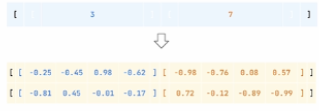
\includegraphics[width=0.65\textwidth]{IMAGES/immagine_2025-02-27_123548078.png}
    \caption[Quantized representation collision]{Example of vectors with the same quantized representation. Source: DeepLearning.AI.\footnotemark.}
    \label{fig:Overfetching}
\end{figure}
\footnotetext{\url{https://learn.deeplearning.ai/courses/retrieval-optimization-from-tokenization-to-vector-quantization/lesson/1/introduction}}
\section{Memory Impact of Quantization in Vector Databases}
Quantization optimizes memory usage in large-scale vector databases by reducing precision. Common techniques include:
\begin{itemize}
    \item \textbf{Scalar Quantization (SQ):} Converts 32-bit floating-point values to 8-bit integers, reducing storage size by a factor of 4.
    \item \textbf{Product Quantization (PQ):} Splits vectors into subvectors, assigns each to a centroid, and stores them as small fixed-size codes (e.g., 1-byte indices). This significantly reduces memory usage but increases indexing complexity.
    \item \textbf{Binary Quantization:} Maps floating-point values to a single bit per value, maximizing compression but sacrificing accuracy.
\end{itemize}

By default, an \textbf{OpenAI embedding} with 1,536 dimensions requires approximately \textbf{6KB per vector}. Applying \textbf{SQ} reduces this to \textbf{1.5KB}, while \textbf{PQ} achieves \textbf{10x or greater compression}, balancing memory efficiency with computational overhead and potential precision loss. The choice of quantization technique depends on the trade-off between storage savings, search latency, and retrieval accuracy.
\section{Experimentation with the quantization techniques}
The Figures below show the disk storage impact and query performance across different embedding formats for the Paper dataset, which consists of 2 million vectors (200 dimensions, float32) evaluated over 100k queries. The experiment has been performed on the VDBMS Weaviate.
\begin{figure}[h]
    \centering
    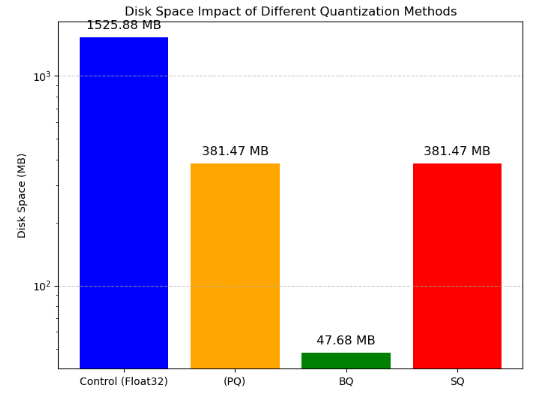
\includegraphics[width=0.4\textwidth]{IMAGES/immagine_2025-02-25_105819873.png}
    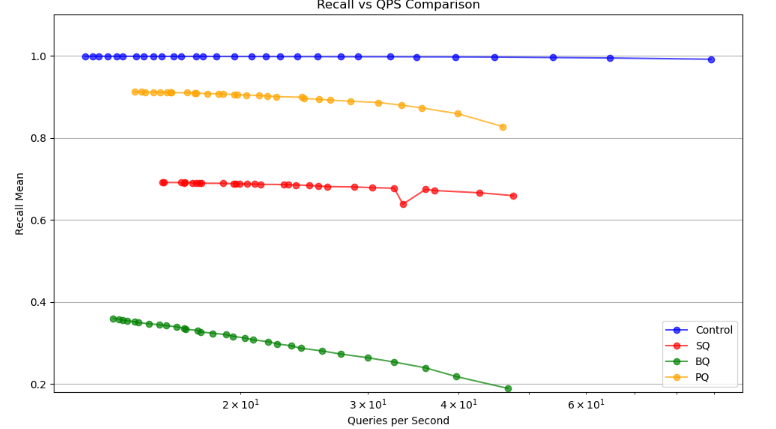
\includegraphics[width=0.4\textwidth]{IMAGES/immagine_2025-02-25_105043241.png}
    \caption{Disk usage and performance difference between the different techniques.}
    \label{fig:Disk Impact}
\end{figure}










\chapter{Indexes}
\label{chap:Indexes in VBDMS}
This chapter will shed light on the indexing aspect of Vector Database Management Systems, specialized data structures that intelligently organize vectors by leveraging their mathematical properties. Their purpose is to optimize the retrieval process that assists search algorithms by improving their performance. There is no index that is tailored for all use cases; each index has been designed with their advantage and disadvantages, the only thing that different approaches have in common is to assist (especially in the large-scale context) reducing the search complexity to sublinear levels.

\section{Flat Index}
The flat index is the simplest approach for vector storage; it involves storing the vectors directly, meaning that queries are always an exact k-nearest neighbors (kNN) search, where the query vector is compared to every other vector in the collection. This approach has limited scalability, as the search speed begins to decline as the vector collection grows. The flat index is best suited for use cases with a manageable collection size, where search accuracy takes priority over search speed.

\section{LSH with Random Projection}
The Locality-Sensitive Hashing (LSH) indexing technique maps high-dimensional vectors to low-dimensional representations by leveraging hash functions that preserve locality and distribution. Vectors that are close in the original space are more likely to share the same hash value. This approach intentionally creates collisions to facilitate efficient retrieval of similar vectors, using hyperplanes as partitioning boundaries.
\begin{figure}[h]
    \centering
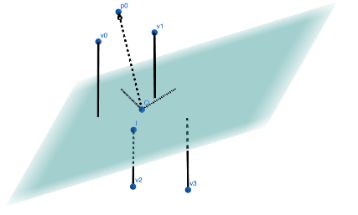
\includegraphics[width=0.35\textwidth]{IMAGES/immagine_2025-02-27_130242965.png}
    \caption[Hyperplane]{Example of Hyperplane. Source: Sofrwaredoug.\footnotemark.}
    \label{fig:Random Projection}
\end{figure}
\footnotetext{\url{https://softwaredoug.com/blog/2023/08/21/implementing-random-projections}}
\end{figure}
A hyperplane splits the vector space into two regions: a positive side and a negative side. To determine which side a vector resides on, the dot product between the vector and a normal vector (perpendicular to the hyperplane) is computed.

The dot product of two vectors $\vec{a} = (a_1, a_2, \dots, a_n)$ and $\vec{b} = (b_1, b_2, \dots, b_n)$ is:

\[
\vec{a} \cdot \vec{b} = \sum_{i=1}^{n} a_i b_i = a_1b_1 + a_2b_2 + \dots + a_nb_n
\]

\begin{itemize}
    \item If the dot product is \textbf{positive}, the vector is assigned a label of \textbf{1} (positive side).  
    \item If the dot product is \textbf{negative}, the vector is assigned a label of \textbf{0} (negative side).  
\end{itemize}

By applying multiple hyperplanes, we create a hashed representation of vectors as binary sequences (composed of 0s and 1s), significantly reducing storage requirements. With $N$ random hyperplanes, each vector is represented as an $N$-bit binary code indicating on which side of each hyperplane it falls.

To measure similarity between vectors, we compute their \textbf{Hamming distance}, which is the number of differing bits between their binary codes.  
\begin{itemize}
    \item A Hamming distance of \textbf{0} indicates that both vectors fall into the same region, meaning no hyperplane separated them.  
    \item Larger Hamming distances indicate greater dissimilarity.
\end{itemize}

Additionally, random projections can be visualized as an \textbf{LSH Tree}, where each hyperplane acts as a decision node, branching into two possible paths: positive or negative. Traversing the tree based on these binary splits results in an efficient search structure for approximate nearest-neighbor queries.

\section{Inverted File Index (IVF)}
The \textbf{Inverted File Index} (IVF) is an indexing technique designed to enhance Approximate Nearest Neighbor (ANN) search performance. IVF partitions the vector space into centroids and limits searches to specific regions, making it ideal for large-scale, high-dimensional applications.

\subsection{Clustering and Voronoi Cells}
A predefined number of centroids is established before clustering, creating an inverted index that associates each vector with its nearest centroid. Once clustering is complete, clusters expand until they form \textit{Voronoi cells}, where each vector belongs to a single cell, defined by the shortest distance to its centroid.
\begin{figure}[h]
    \centering
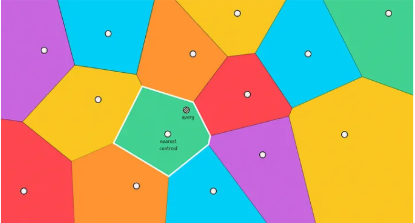
\includegraphics[width=0.55\textwidth]{IMAGES/immagine_2025-02-27_130909576.png}
    \caption[Voronoi Cells]{Example of Voronoi cells. Source: Towardsdatascience.\footnotemark[2]}
    \label{fig:Voronoi}
\end{figure}
\footnotetext[2]{\url{https://towardsdatascience.com/similarity-search-knn-inverted-file-index-7cab80cc0e79}}
\subsection{Querying and the Edge Problem}
Queries locate the nearest centroids and search for the closest vectors within them. However, the \textbf{edge problem} arises when suitable vectors near Voronoi boundaries are ignored. This issue worsens in high dimensions as cell boundaries become less distinct. To mitigate this, querying multiple cells increases recall at the cost of speed.
\begin{figure}[h]
    \centering
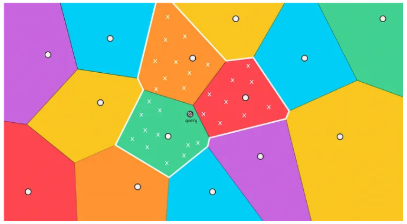
\includegraphics[width=0.55\textwidth]{IMAGES/immagine_2025-02-27_131611893.png}
    \caption[Edge problem]{Edge problem. Source: Towardsdatascience.\footnotemark[2]}
    \label{fig:VoronoiEdges}
\end{figure}
\subsection{IVF Variants}
The basic form of IVF, known as \textbf{IVFFlat}, performs a brute-force search within identified cells. Advanced variants such as \textbf{IVFPQ} (Product Quantization) and \textbf{IVFSQ} (Scalar Quantization) compress vector representations, enhancing scalability and reducing memory usage. These techniques will be covered in the next chapter.


\section{Navigable Small Worlds}
The NSW index consists of a graph that contains both long-range and short-range links. It is based on the “small world” or "six degrees of separation" rule, where each entity is, on average, separated by six degrees of link separation. This structure exhibits a high degree of clustering, where nodes are grouped into tightly-knit communities, yet only a few steps are needed to traverse between two different nodes. Essentially, this allows nodes that are typically "far" from each other in other graph-based structures to reach one another in just a few steps. Each node represents an item and maintains a friend list containing other vertices to which it is connected. This solution is fast but not highly accurate and requires tuning to perform well in ANN search over high-dimensional spaces.

\subsection{Construction}
Unlike some other indexes, the construction of the index is not a deterministic process, at first the dataset is shuffled and then the nodes are sequentially created. The main parameters in this process is  \textbf{M} which the maximum number of connections a node can have. As nodes are inserted it gets connected to nearest nodes based on a distance metrics like the cosine distance.

\begin{figure}[h]
    \centering
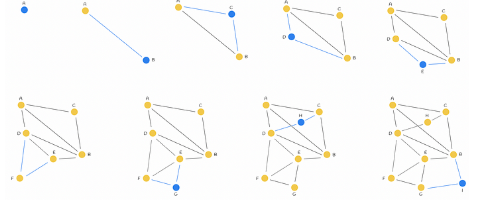
\includegraphics[width=0.55\textwidth]{IMAGES/immagine_2025-02-27_132644429.png}
    \caption[NSW construction]{Example of NSW construction with M=2. Source: Towardsdatascience.\footnotemark.}
    \label{fig:NSW}
\end{figure}
\footnotetext{\url{https://www.deeplearning.ai/short-courses/vector-databases-embeddings-applications/ }}

\subsection{Graph traversal}
The search begins by selecting a vertex as the entry point. It then performs a greedy search, determining the next vertex to move to by checking the current vertex’s friend list and moving to the closest vertex to the query node. The search terminates when no closer node is found.  
Since this search strategy is inherently greedy, it attempts to reach the global optimal solution by making the best local decision at each step. While this approach is simple and fast, it is susceptible to early stopping, where the search gets trapped in regions of the graph where the local optimum has no better neighboring candidates.  
To mitigate the risk of getting stuck in dead regions, various strategies can be employed. One such method is \textbf{“beam search"}, which maintains a \textbf{top-k} list of the best candidates at each step. Another approach is “multi-hop search,” which considers not only direct neighbors but also neighbors of neighbors.
\begin{figure}[h]
    \centering
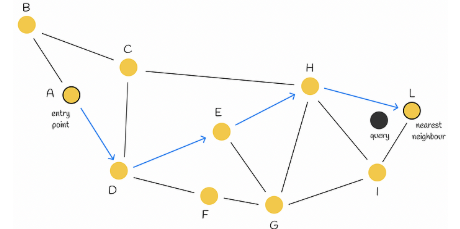
\includegraphics[width=0.6\textwidth]{IMAGES/immagine_2025-02-27_132919654.png}
    \caption[NSW routing]{example of NSW routing where A is entry point. Source: DeepLearningAI.\footnotemark.}
    \label{fig:NSW traversal}
\end{figure}
\footnotetext{\url{https://www.deeplearning.ai/short-courses/vector-databases-embeddings-applications/ }}

\section{Hierarchical Navigable Small Worlds}
The HNSW index is an evolution of the \textbf{Navigable Small World (NSW)} graph, incorporating principles from the probabilistic data structure known as the \textbf{skip list}. A skip list consists of multiple layers of ordered linked lists, where each upper layer contains a subset of elements from the layer below. This hierarchical structure enables efficient search by starting from the topmost layer and performing a sequential search.  
\begin{figure}[h]
    \centering
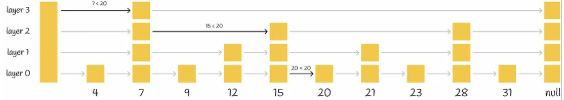
\includegraphics[width=0.8\textwidth]{IMAGES/immagine_2025-02-27_133448847.png}
    \caption[Skip List]{Skip List. Source: Towardsdatascience.\footnotemark[2]}
    \label{fig:Skip List}
\end{figure}

If the target element is found, the search terminates. Otherwise, upon encountering a greater value, the algorithm descends to the next layer, using the previously visited element as the new entry point.  


The \textbf{HNSW} index follows a similar layered structure, where:
\begin{itemize}
    \item The \textbf{topmost layer} contains a small subset of representative nodes.
    \item The \textbf{in-between layers} contain progressively more nodes.
    \item The \textbf{lowest layer} includes all nodes in the dataset.
\end{itemize}
\begin{figure}[h]
    \centering
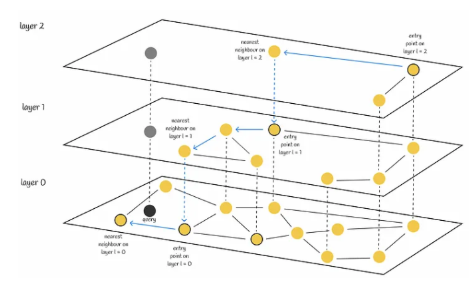
\includegraphics[width=0.7\textwidth]{IMAGES/immagine_2025-02-27_133909960.png}
    \caption[HNSW]{HNSW index. Source: Towardsdatascience.\footnotemark[2]}
    \label{fig:HNSW}
\end{figure}
This multi-layered organization significantly improves retrieval efficiency by reducing the number of comparisons required for nearest neighbor search.  

\subsection{Search Process}  

The HNSW query process is similar to NSW but introduces a hierarchical search mechanism. After locating the nearest node in a layer, it serves as the entry point for the lower layer.  

HNSW graphs follow the skip list principle:  
\begin{itemize}  
    \item The \textbf{topmost layer} has fewer nodes and connections.  
    \item Lower layers have increasing connectivity until \textbf{Layer 0}, which contains all data points.  
\end{itemize}  

The search begins at a predefined entry node in the top layer and performs a greedy search. The algorithm descends to the next layer when it finds a closer node in that layer. This process continues until reaching Layer 0, ensuring all potential nearest neighbors are considered.  

HNSW search is controlled by key parameters:  
\begin{itemize}  
    \item \textbf{$ef$ (exploration factor)}: Determines the number of candidate nodes kept during the search. A higher $ef$ improves recall at the cost of increased latency. 
    \item \textbf{Entry Point Selection}: The algorithm selects a fixed or dynamically chosen entry node in the topmost layer to begin the search.  
\end{itemize}  

These parameters allow fine-tuning of search accuracy, efficiency, and resource usage in HNSW-based vector searches.  
\subsubsection{Impact of M parameter on HNSW search}
The Figures below show the impact of different values of M,performed over the embedding that come from the Tripclick dataset, which consists rhoughly of 800k vectors (768 dimensions, float32) evaluated over 1000 queries. The experiment has been performed on the VDBMS Weaviate.
\begin{figure}[h]
    \centering
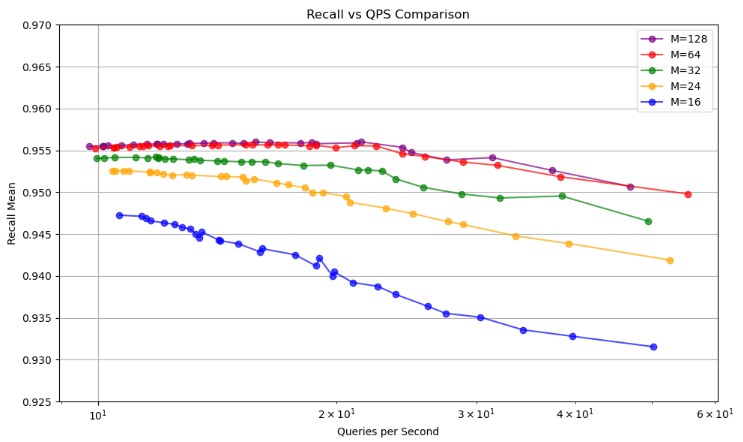
\includegraphics[width=0.7\textwidth]{IMAGES/immagine_2025-02-27_142057404.png}
    \caption[Analysis of M parameter]{QPS vs Recall between different values of M.}
    \label{fig:M search}
\end{figure}

\subsection{Construction Process of HNSW}
The construction of an \textbf{HNSW} index follows a hierarchical approach, inspired by skip lists, to optimize approximate nearest neighbor search. The graph is built incrementally, adding one data point at a time while maintaining efficient connectivity across multiple layers.
\subsubsection*{Key Parameters}
The construction process is governed by several key parameters:
\begin{itemize}
    \item \textbf{Maximum Layer ($L_{\max}$):}  
    Determines the highest level a node can be assigned. It is typically chosen using a logarithmic distribution based on the dataset size.

    \item \textbf{Maximum Connections per Layer ($M$):}  
    Defines the number of bidirectional edges each node can maintain per layer, balancing search efficiency and memory usage.

    \item \textbf{Connectivity Factor (efConstruction):}  
    Controls the number of nearest neighbors considered during graph construction. A higher value results in better graph quality but increases indexing time.

    \item \textbf{Insertion Strategy:}  
    Each new data point is assigned a random layer up to $L_{\max}$ and inserted into the graph by connecting to its $M$ nearest neighbors in each layer.

    \item \textbf{Pruning Strategy:}  
    Redundant edges are removed to ensure efficient navigation while maintaining strong graph connectivity.
\end{itemize}

\subsubsection*{Construction Algorithm}

\begin{enumerate}
    \item Assign each new data point a layer up to $L_{\max}$.
    \item Insert the point into the topmost layer and connect it to the $M$ nearest neighbors.
    \item Repeat the process for each lower layer, ensuring bidirectional edges.
    \item Apply pruning to maintain an optimal balance between connectivity and efficiency.
\end{enumerate}

The hierarchical structure ensures that higher layers facilitate fast exploration, while lower layers refine the search for precise nearest neighbors.


 
\section{DiskANN}
One of the main drawback of graph-based indexes like NSW and HNSW, is the significant memory footprint, which makes querying over large amount of data expensive. While this may not be an issue in distributed and high resources environments, the same cannot be said for single machines with limited memory. The most basic approaches for handling single node environments are the employment of \textbf{IVFPQ} or by sharding the dataset with their own in-memory indexes which during the search each result is merged together. These solution suffer from a lower recall and to address this, \textbf{DiskANN} provides an SSD resident index with the objective of reducing the memory footprint and optimize disk accesses thanks to the assistance of the \textbf{Vamana} algorithm, which differentiates itself from NSW by constructing the graph in order to optimize disk access instead of improved traversal.

\subsection{Graph Construction Process}
Instead of starting with a sparse graph and gradually adding edges (as in NSW), Vamana begins with a dense graph and iteratively prunes unnecessary edges. The process consists of the following steps:

\begin{enumerate}
    \item \textbf{Initialize:}  
    Start with a randomly connected graph with excess edges.  

    \item \textbf{Graph Construction:}  
    For each point $p$:  
    \begin{enumerate}
        \item \textbf{Find Nearest Neighbors:} Greedy search in the current graph.  
        \item \textbf{Prune Edges:} Remove redundant connections while ensuring connectivity.  
        \item \textbf{Add Backward Links:} Ensure bidirectional edges for efficient traversal.  
    \end{enumerate}

    \item \textbf{Refinement:}  
    Perform two rounds of pruning with different distance thresholds to optimize local and long-range connections.  

    \item \textbf{Disk Optimization:}  
    Store the graph efficiently to minimize random disk access and enable batched reads.  
\end{enumerate}
This pruning-based method enables Vamana to optimize the trade-off between \textbf{graph diameter}, which influences search depth, and \textbf{node degree}, which impacts memory consumption, more efficiently than conventional techniques. DiskANN utilizes Vamana because it builds a \textbf{flat graph}, making it more suitable for disk storage compared to hierarchical structures.
\begin{figure}[h]
    \centering
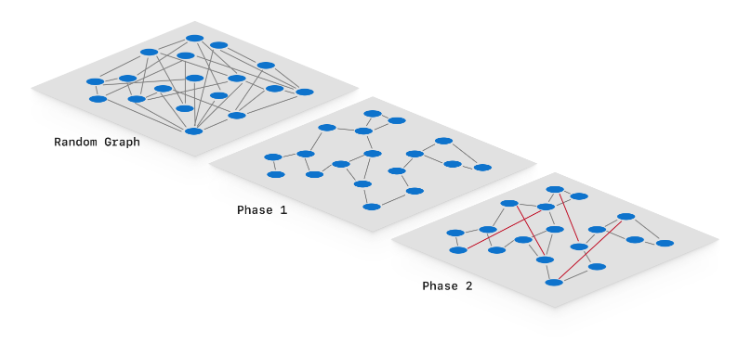
\includegraphics[width=0.7\textwidth]{IMAGES/immagine_2025-02-27_134619701.png}
    \caption[Vamana]{Vamana Graph example. Source: Planetscale.\footnotemark.}
    \label{fig:Vamana}
\end{figure}
\footnotetext{\url{https://planetscale.com/docs/vectors/terminology-and-concepts
}}
\subsection{Optimizations in DiskANN}
DiskANN provides some optimization in order to increase querying performance:

\begin{itemize}
    \item \textbf{Caching:} Nodes that are fetched more freqeuntly than others are stored in RAM, in order to reduce SSD use and increase the performance.
    \item \textbf{Compressed vectors and re-ranking:} In order to increase retrieval efficiency, vectors are stored in RAM in their compressed form, in order to do a preliminary comparison. After, a re-ranking process is done with a full precision SSD search.
    \item \textbf{Clustered Indexing:} Partitions data into overlapping clusters using k-means clustering. Each data point belongs to multiple clusters, ensuring connectivity for search algorithms.
    \item \textbf{Beam Search:} Retrieves neighborhood data from SSD in small batches, reducing read latencies by grouping nearby data access requests.
\end{itemize}
\clearpage
